\documentclass[12pt]{article}
\usepackage[utf8]{inputenc}
\usepackage[T1]{fontenc}
\usepackage[polish]{babel}
\usepackage{geometry}
\usepackage{tabularx}
\usepackage[table,xcdraw,dvipsnames]{xcolor}
\usepackage{tabularx}
\usepackage{color}
\usepackage{subfig}
\usepackage{sidecap}
\usepackage{wrapfig}
\usepackage{float}
\usepackage{enumerate}
\usepackage{graphicx}
\usepackage{multirow}
\usepackage{hyperref}
\usepackage{titlesec}
\usepackage{amsmath}
\usepackage{anyfontsize}
\usepackage{indentfirst}
\usepackage{listings}
\usepackage{multicol}
\usepackage{pgfplots}
\usepackage{fancyhdr}

\newgeometry{tmargin=1.8cm,bmargin=1.8cm,lmargin =1.8cm,rmargin=1.8cm}
\begin{document}

\newcommand{\zdjecie}[3]
{
    \begin{figure}[H]
        \renewcommand{\figurename}{Rys.}
        \centering
        \includegraphics[width=\textwidth]{#1}
        \caption{#2}
        \label{#3}
    \end{figure}
}

\begin{table}[H]
    \centering
    \renewcommand{\arraystretch}{1.5}
    \begin{tabularx}{\textwidth}{|X|X|}
    \hline
    \multicolumn{2}{|c|}{\large\textbf{Notatka służbowa nr 4}} \\ \hline
    Temat:          & Regulator PID na sterowniku VersaMax    \\ \hline
    Wykonanie:      & Zuzanna Mejer, 259382   \\ \hline
    Termin zajęć:   & poniedziałek TP, 10:55  \\ \hline  
    Data:           & 16.12.2022    \\ \hline
    \end{tabularx}
    \end{table}

\section{Cel ćwiczenia}
Celem ćwiczenia było utworzenie projektu regulacji PID oraz analiza wykresów regulacji. Ćwiczenie wykonano na sterowniku PLC VersaMax z wykorzystaniem programu Proficy Machine Edition 8.0. 


\section{Uruchomienie oprogramowania i konfiguracja sterownika}
Przed rozpoczęciem pracy na sterowniku, należało uruchomić oprogramowanie Proficy Machine Edition i skonfigurować sterownik. W tym celu wykonano poniższe czynności:
\begin{enumerate}
    \item Utworzono nowy projekt wybierając z głównego menu \textit{File $\rightarrow$ New Project}. Wpisano tytuł projektu oraz wybrano szablon \textit{GE Intelligent Platform VersaMax PLC} (rys. \ref{nowy_projekt}). Poprawnie utworzony projekt widoczny w zakładce \textit{Navigator} przedstawiono na rys. \ref{utworzony_projekt}.
    \zdjecie{./zdj/nowy_projekt.png}{Utworzenie nowego projektu w programie Proficy Machine Edition}{nowy_projekt}
    \zdjecie{./zdj/utworzony_projekt.png}{Poprawnie utworzony projekt}{utworzony_projekt}
    \item Rozwijając \textit{Hardware Configuration $\rightarrow$ Main Rack} pokazały się moduły sterownika. Najpierw, klikając na moduł \textit{PWR} prawym klawiszem i wybierając \textit{Replace Module}, uzupełniono nazwę modułu jako \textit{IC200PWR002/012} (rys. \ref{CPU}). O poprawności wybrania modułu PWR świadczy pojawienie się zielonego elementu przy ikonie, co przedstawia rys. \ref{CPU2}.
    \zdjecie{./zdj/CPU.png}{Zamiana modułu PWR}{CPU}
    \zdjecie{./zdj/CPU2.png}{Poprawnie wybrana jednostka PWR - zielony element przy ikonie}{CPU2}
    \item Rzeczywisty sterownik posiadał 3 ,,kasety''. W programie domyślnie pojawia się klasyczna jednostka centralna jako Slot 0, którą trzeba było zamienić za pomocą opcji \textit{Replace Module} z IC200CPU001 na IC200CPUE05. Pozostałe 2 ,,kasety'' należało dodać najpierw wybierając podstawkę (opcja \textit{Add Carrier/Base}) - rys. \ref{podstawka}, a następnie wybierając właściwy moduł opcją \textit{Add Module} - rys. \ref{modul}. W ten sposób zostały zdefiniowane poszczególne ,,kasety'': \\
    Slot 1 $\rightarrow$ IC200MDD845 \\
    Slot 2 $\rightarrow$ IC200ALG430. 
    \zdjecie{./zdj/podstawka.png}{Przykład wybranej podstawki}{podstawka}
    \zdjecie{./zdj/modul.png}{Przykład wybranego modułu}{modul}
    \item Następnie wykonano konfigurację jednostki centralnej, to znaczy: zdezaktywowano hasło (rys. \ref{haslo}), uzupełniono adres IP (rys. \ref{IP}) oraz maskę (rys. \ref{maska}), oraz przeniesiono obszar pamięci statusu od adresu początkowego $\%I100$ (rys. \ref{adresy}).
    \zdjecie{./zdj/haslo.png}{Zdezaktywowanie hasła}{haslo}
    \zdjecie{./zdj/IP.png}{Zmiana adresu IP}{IP}
    \zdjecie{./zdj/maska.png}{Uzupełnienie maski}{maska}
    \zdjecie{./zdj/adresy.png}{Przeniesienie obszaru pamięci statusu}{adresy}
    \item Zmieniono adres referencyjny dla wejść binarnych od $\%I001$ (rys.\ref{adresy_binarne}).
    \zdjecie{./zdj/adresy_binarne.png}{Zmiana adresów obszaru pamięci dla wejść binarnych}{adresy_binarne}
    \item Po zakończeniu konfiguracji sprzętowej przeprowadzono walidację projektu (rys. \ref{walidacja}).
    \zdjecie{./zdj/walidacja}{Walidacja projektu}{walidacja} 
\end{enumerate}


\section{Program do regulacji PID}
\subsection{Program w języku drabinkowym}
W celu przeprowadzenia badania odpowiedzi skokowych regulatora PID wprowadzony został następujący program w sekcji \textit{Logic $\rightarrow$ Program Blocks $\rightarrow$ MAIN}:

\begin{figure}[H]
    \centering
    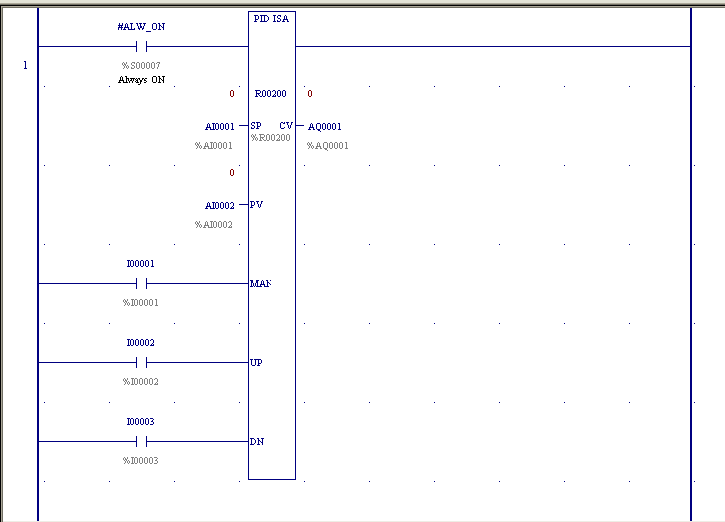
\includegraphics[width = \textwidth]{./zdj/network1.png}
\end{figure}
\begin{figure}[H]
    \centering
    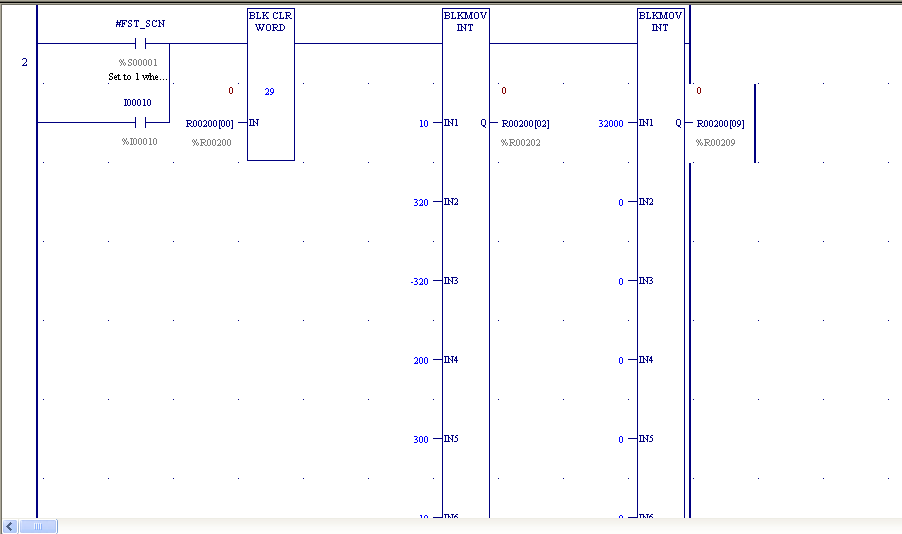
\includegraphics[width = \textwidth]{./zdj/network2.png}
\end{figure}
\begin{figure}[H]
    \centering
    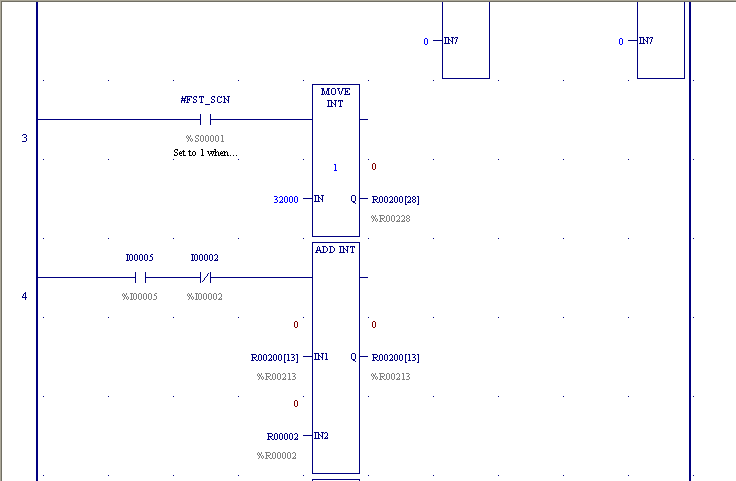
\includegraphics[width = \textwidth]{./zdj/network3.png}
\end{figure}
\begin{figure}[H]
    \centering
    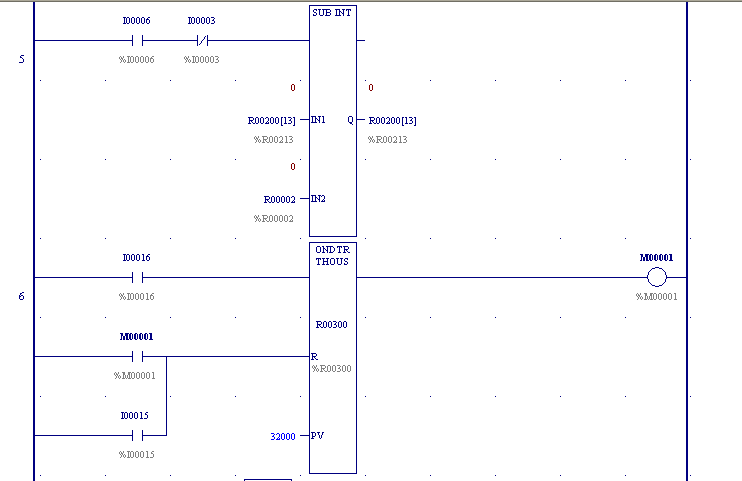
\includegraphics[width = \textwidth]{./zdj/network4.png}
\end{figure}

\zdjecie{./zdj/network5.png}{Program regulatora PID w języku drabinkowym}{}


\subsection{Uruchomienie i działanie programu}
Po powtórzeniu walidacji całego programu, przesłano go do sterownika. Przed poleceniem połączenia wybrano port fizyczny komputera Ethernet i wpisano adres IP sterownika (rys.\ref{inspector}).
\zdjecie{./zdj/inspector}{Port fizyczny Ethernet i adres IP}{inspector}
Przesyłanie rozpoczyna się od otwarcia okna \textit{Download to Controller} (rys.\ref{download}), następnie pojawia sie okno \textit{Start Controller} (rys.\ref{start}).
\zdjecie{./zdj/download.png}{\textit{Download to Controller}}{download}
\zdjecie{./zdj/start}{\textit{Start Controller}}{start}


\section{Analiza przebiegów}
\subsection{Regulator PI}
Poprawność działania regulacji całkującej sprawdzono dla następujących danych: współczynnik wzmocnienia $K_p=1$, czas zdwojenia $T_i = 100s$ oraz $T_i = 10s$. Na wejście podano skok jednostkowy i uzyskano następujące przebiegi:

\zdjecie{./zdj/calkujacy_100.png}{Odpowiedź regulatora PI przy $T_i=100s$}{PI_100}
\zdjecie{./zdj/calkujacy_10.png}{Odpowiedź regulatora PI przy $T_i=10s$}{PI_10}

\subsection{Regulator PD}
Poprawność działania regulacji różniczkującej sprawdzono dla następujących danych: współczynnik wzmocnienia $K_p=1$, czas wyprzedzenia $T_d = 15s$ oraz $T_d = 10s$. Na wejście podano sygnał narastający liniowo i uzyskano następujące przebiegi:

\zdjecie{./zdj/rozniczkujacy_15.png}{Odpowiedź regulatora PD przy $T_d=15s$}{PD_15}
\zdjecie{./zdj/rozniczkujacy_10.png}{Odpowiedź regulatora PD przy $T_d=10s$}{PD_10}

\section{Podsumowanie}


\end{document}